\chapter{绪论}
\section{研究背景}
近年来,深度学习技术,特别是深度神经网络在图像识别领域取得了突破性进展。本节将概述这一领域的发展历程和最新研究动态\cite{krizhevsky2012imagenet,goodfellow2014generative}。

\section{研究意义}
提高图像识别的准确性和效率对于许多实际应用至关重要,如医疗诊断、自动驾驶等。本研究旨在推动这一领域的发展,并探索新的应用方向。



\begin{table}[htbp]
    \centering
    \bicaption{示例表格}{Example table}\label{tab:example}
    \begin{tabular}{|l|p{5cm}|p{5cm}|}
        \hline
        \textbf{网络类型} & \textbf{主要特点} & \textbf{典型应用} \\
        \hline
        卷积神经网络 (CNN) &
        \begin{itemize}
            \item 局部感受野
            \item 权值共享
            \item 多层结构
        \end{itemize} &
        \begin{itemize}
            \item 图像识别
            \item 物体检测
            \item 人脸识别
        \end{itemize} \\
        \hline
        循环神经网络 (RNN) &
        \begin{itemize}
            \item 具有记忆能力
            \item 可处理序列数据
            \item 存在梯度消失问题
        \end{itemize} &
        \begin{itemize}
            \item 自然语言处理
            \item 语音识别
            \item 时间序列预测
        \end{itemize} \\
        \hline
        长短时记忆网络 (LSTM) &
        \begin{itemize}
            \item RNN的变体
            \item 解决长期依赖问题
            \item 具有门控机制
        \end{itemize} &
        \begin{itemize}
            \item 机器翻译
            \item 文本生成
            \item 情感分析
        \end{itemize} \\
        \hline
    \end{tabular}
\end{table}


\begin{figure}[h]

    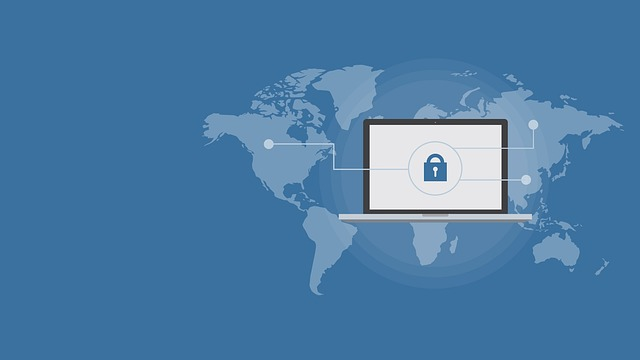
\includegraphics[width=\textwidth]{figures/example.jpg}
    \bicaption{示例图片}{Example pictures}\label{fig:example}
\end{figure}
